\documentclass{standalone}
\usepackage{tikz}

\begin{document}

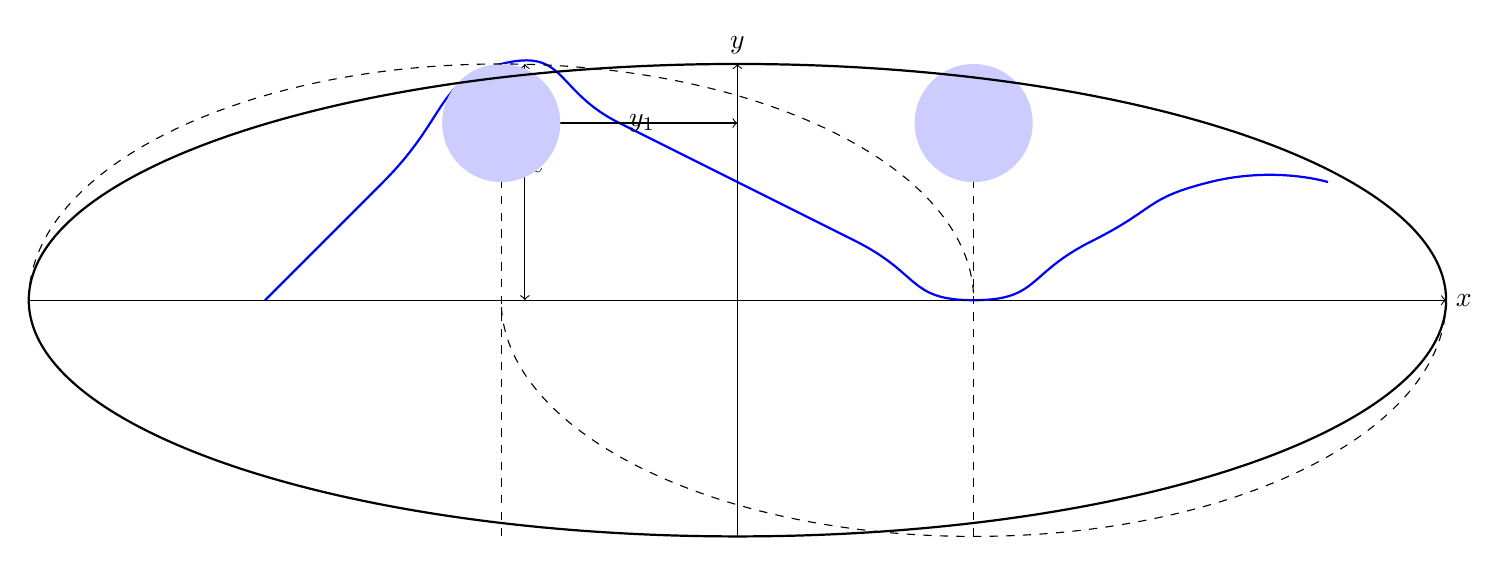
\begin{tikzpicture}[scale=1.5]
    % Draw the x-axis
    \draw[->] (-6,0) -- (6,0) node[right] {$x$};
    
    % Draw the y-axis
    \draw[->] (0,-2) -- (0,2) node[above] {$y$};
    
    % Draw the curve
    \draw[thick, blue] plot [smooth, tension=1] coordinates {(-4,0) (-3,1) (-2,2) (-1,1.5) (0,1) (1,0.5) (2,0) (3,0.5) (4,1) (5,1)};
    
    % Draw the horizontal line at y=0
    \draw[dashed] (-6,0) -- (6,0);
    
    % Draw the vertical lines to indicate the cross-section
    \draw[dashed] (-2,-2) -- (-2,2);
    \draw[dashed] (2,-2) -- (2,2);
    
    % Label the cross-section
    \node at (-2, 1.5) [circle,fill,inner sep=1.5pt]{};
    \node at (2, 1.5) [circle,fill,inner sep=1.5pt]{};
    
    % Label the width of the cross-section
    \draw[<->] (-1.8,2) -- node[above] {$\Delta x$} (-1.8,0);
    
    % Label the height of the cross-section
    \draw[<->] (-2,1.5) -- node[right] {$y_1$} (0,1.5);
    
    % Draw the cross-section
    \fill[blue!20] (-2,1.5) circle (0.5cm);
    \fill[blue!20] (2,1.5) circle (0.5cm);
    
    % Draw the full ellipse
    \draw[thick] (-6,0) arc (180:0:6 and 2);
    \draw[thick] (6,0) arc (0:-180:6 and 2);
    
    % Draw the dashed ellipse
    \draw[dashed] (-6,0) arc (180:0:4 and 2);
    \draw[dashed] (6,0) arc (0:-180:4 and 2);
\end{tikzpicture}

\end{document}